\section{Metoder}
    \subsection{Synteser} 
    Med udgangspunkt i den fundne syntesevejledning \parencite{Ole2019} udføres syntesen for ethyl-- og propylparaben grundet deres respektive alkoholers lavewre farlighed end methanol. Af samme grund benyttes ethanol som opløsningsmiddel under oprensningen, idet der herved helt undgås eksponering for methanol hvilket drastisk minimerer eksponeringen for farlige kemikalier under syntesen.

    Det vælges at producere 2 parabener for at muliggøre samligning af deres respektive H--NMR--spektre, og begrunde hvorfor disse er opstået. 

    Derudover giver det også mening jf.\ et eventuelt hæmningsforsøg at fravælge methylparaben da den generelt ses som havende en lavere effektivitet grundet dens ringere evne til at reagere med mikroorganismernes cellemembraner pga.\ større polaritet.

    Et flowdiagram for syntesen udarbejdes for at give overblik over syntesen, samt for at give bedre overblik gennem processen. Flowdiagrammet kan ses under bilag.

    \subsubsection{Syntese 1: Ethylparaben}
    Ca.\ 5g 4-hydroxybenzoesyre afvejes i rundbundet kolbe med slib:
    \begin{figure}[H] \centering
        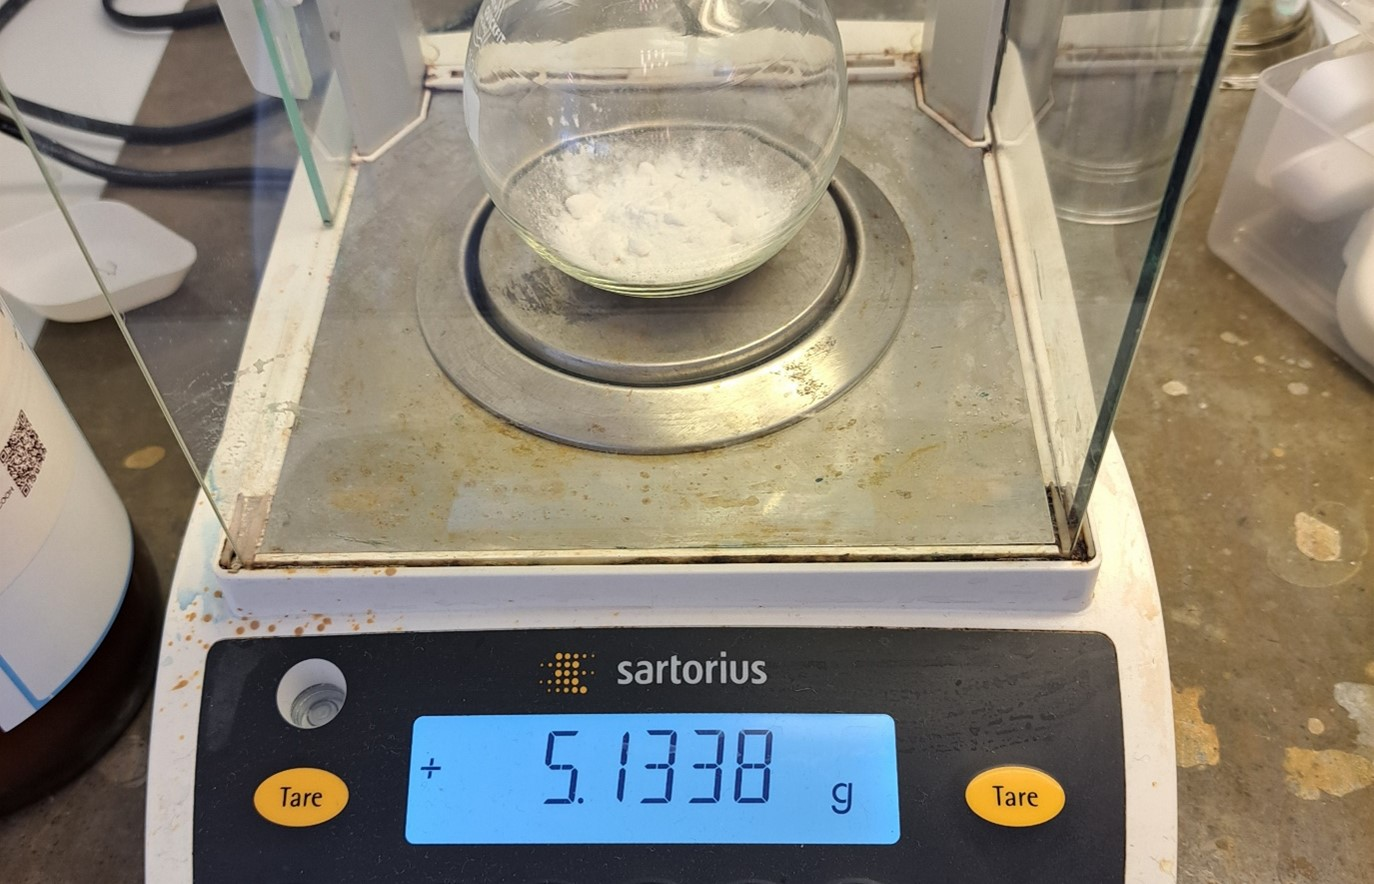
\includegraphics[width=\textwidth]{billeder/afvejning}
        \caption{Afvejning af 4-hydroxybenzoesyre.}
    \end{figure} 
    Da syntesen sker med et overskud af alkohol vil der ideelt ske en fuldstændig reaktion. På baggrund heraf bestemmes det teoretiske udbytte ved at sætte dets stofmængde lig stofmængden af 4-hydroxybenzoesyre:
    \[
        n_{\text{4-hydroxybenzoesyre}}=\frac{5.1338\si{g}}{138.12\si{g \per mol}}=0.037169\si{mol}=n_{\text{ethylparaben}}
    \]
    Den teoretiske stofmængde af dannet ethylparaben omregnes nu til en masse hvorved det fås at:
    \[
        m_{\text{ethylparaben}}=0.037169\si{mol} \cdot 166.17\si{g\per mol}=6.1745g
    \]
    Et regneark udarbejdes til bestemmelsen af det teoretiske udbytte gennem de resterende synteser, en version med værdierne for denne syntese kan ses i bilag 2.

    Der afmåles nu 30mL ethanol i måleglas, hvorefter det overføres til den rundbundede kolbe. Kolben rystes til 4-hydroxybenzoesyren er fuldstændigt opløst, hvorefter 2.5mL svovlsyre tilsættes dråbevist under konstant forsigtig omrystning. Opløsningen placeres i en varmekappe og forsynes med et svalerør for at koge med reflux i ca. 1 time.

    Efter timen er gået slukkes varmekappen, hvorefter opløsningen nedkøles indtil det ikke længere er kogende og overføres til et 250mL bægerglas med 75mL demineraliseret vand. Bægerglasset placeres nu på en kogeplade og tilsættes en magnetomrører, hvorefter der sørges for moderat omrøring. Blandingen bestående af 10\% natriumcarbonat tilsættes nu opløsningen indtil udviklingen af gas stopper, hvorved svovlsyren vil være neutraliseret.

    Idet det ikke indgår i forsøgsvejledningen, udregnes mængden af natriumcarbonat der villet være nødvendig for at neutralisere svovlsyren, dog vil der under processen gøres brug af natriumcarbonat i overskud da det ingen negativ virkning vil have, eftersom temperaturen vil være for lav til at forsæbning af parabenen vil kunnet ske.

    Da svovlsyre har mulighed for at afgive 2 hydroner hvorved det reduceres til dets syrerest-ion, $\mathrm{SO_4^{2-}}$, må den tilsatte base kunnet optage 2 hydroner for at netrualisere 1 svovlsyremolekyle:
    \begin{figure}[H]
        \resizebox{\textwidth}{!}{
        \schemestart
        \chemfig{S(=[1]O)(=[3]O)(-[5]OH)(-[7]OH)}
        \+
        \chemfig{H_{2}O}
        \arrow{->}
        \chemfig{S(=[1]O)(=[3]O)(-[5]OH)(-[7]O^{-})}
        \+
        \chemfig{H^{+}}
        \arrow{->}
        \chemfig{S(=[1]O)(=[3]O)(-[5]O^{-})(-[7]O^{-})}
        \+ 2
        \chemfig{H^{+}}
        \schemestop
        }
        \caption{Dissociering af svovlsyre ved tilsættelse til vand.}
    \end{figure}
    Samtidig er det klart at natriumcarbonat har mulighed for at optage 2 hydroner da det ved tilsættelse til vand øjeblikkeligt dissocierer til natrium- og carbonationer, der herefter reagerer videre for at danne natriumhydroxid.
    \begin{figure}[H]
        \resizebox{\textwidth}{!}{
        \schemestart
        \chemfig{C(=[2]O)(-[5]NaO)(-[7]ONa)}
        \+
        \chemfig{H_{2}O}
        \arrow{->}
        \chemfig{C(-[3]O^{-})(-[5]O^{-})=O}
        \+ 2
        \chemfig{Na^{+}}
        \schemestop
        }
        \caption{Dissociering af natriumcarbonat ved tilsættelse til vand.}
    \end{figure}
    Carbonationen har mulighed for at reagere med vand hvorved der dannes bicarbonat og en hydroxidion, bicarbonationen reagerer videre med vand for at danne ustabil kulsyre og endnu en hydroxidion, hvorefter den ustabile kulsyre brydes hvilket medfører dannelsen af carbondioxid og vand. 
    \begin{align}
        \mathrm{CO_3^{2-} + H_2O} &\longrightarrow \mathrm{HCO_3^- + OH^-} \\
        \mathrm{HCO_3^- + H_2O} &\longrightarrow \mathrm{H_2CO_3 + OH^-} \\
        \mathrm{H_2CO_3} &\longrightarrow \mathrm{CO_2 + H_2O}
    \end{align}
    De dannede hydroxidioner har nu mulighed for at reagere med hydronerne dannet af svovlsyren, mens natriumionerne har mulighed for at reagere med sulfationerne.
    \begin{align*}
        \mathrm{OH^- + H^}+ &\longrightarrow \mathrm{H_2O} \\
        \mathrm{2Na^+ + SO_4^{2-}} &\longrightarrow \mathrm{Na_2SO_4}
    \end{align*}
    Dette muliggør opskrivning som en totalreaktion ved:
    \begin{figure}[H]
        \resizebox{\textwidth}{!}{
        \schemestart
        \chemfig{C(=[2]O)(-[5]NaO)(-[7]ONa)}
        \+
        \chemfig{S(=[1]O)(=[3]O)(-[5]OH)(-[7]OH)}
        \arrow{->}
        \chemfig{S(-ONa)(-[4]NaO)(=[2]O)(=[6]O)}
        \+
        \chemfig{C(=O)(=[4]O)}
        \+ 2
        \chemfig{H_{2}O}
        \schemestop
        }
        \caption{Totalreaktion mellem svovlsyre og natriumcarbonat i vandig opløsning.}
    \end{figure}
    Da det nu er klart at reaktionen mellem svovlsyre og natriumcarbonat foregår i forholdet 1:1 og at der under syntesen benyttes 2.5mL svovlsyre med en densitet på $1.84\si{g \per mL}$ må det være nødvendigt at bruge:
    \[
        n_{\text{svovlsyre}}=\frac{2.5\si{mL} \cdot 1.84\si{g\per mL}}{98.08\si{g\per mol}}=0.04690mol
    \]
    natriumcarbonat til at neutralisere svovlsyren. Stofmængden omregnes til en masse af natriumcarbonat, her er det vigtigt at pointere at der benyttes natriumcarbonatdecahydrat under fremstillingen af opløsningen, grundet dets effekt på molvægten.
    \[
        m_{\text{natriumcarbonat}}=0.04690\si{mol} \cdot 286.14\si{g\per mol}=13.4200\si{g}
    \]
    Da det ikke skaber et problem at tilsætte natriumcarbonat i overskud laves opløsning ved brug af 15g natriumcarbonatdecahydrat og 135g vand. En 10\% opløsning benyttes for at reducere voldsomheden af reaktionen mellem den stærke syre og base, samt for at modvirke dens store eksotermicitet.

    Den neutraliserede opløsning sugefiltreres og skylles 3 gange med demineraliseret vand efter kort tids afkøling. Det isolerede krystallinske stof overføres til et 250mL bægerglas. Samtidigt opvarmes 50mL hhv.\ ethanol og vand til opvarmning i hvert deres bægerglas. Når ethanolen koger opløses det krystallinske stof i så lidt som muligt hvorefter varmt vand tilsættes til opløsningen bliver uklar.

    Opløsningen stilles nu til frivillig nedkøling, hvorved parabenen igen udfældes og kan isoleres ved sugefiltrering i afvejet glasfilterdigel. Det dannede produkt stilles til tørring i glasfilterdiglen benyttet til filtreringen.

    \subsubsection{Syntese 2: Propylparaben}
    

    \subsubsection{Syntese 3: Dobbeltsyntese}
        

    \subsection{Smeltepunktsbestemmelse}
    

    \subsection{NMR--spektroskopi}
    

    \subsection{IR--spektroskopi}
    

    \subsection{Hæmningsforsøg}
    Et hæmningsforsøg udføres også for at undersøge parabenernes hæmmende vækst på forskellige bakterier.Med udgangspunkt i litteraturen er det klart at parabener er mere effektive mod Gram--positive end Gram--negative bakterier \parencite{Joao2021}. Derudover har tidligere studier undersøgt de effektive koncentrationer for væksthæmning ved de forskellige parabener for bakteriearterne \parencite{Wies2019}. 

    Grundet dette undersøges 2 forskellige bakterier, \textit{bacilius cereus} og \textit{escherichia coli}, for at muliggøre undersøgelse af både et gram--positivt og gram--negativt bakterie:
    \begin{table}[H]\centering
        \caption{Karakteristika, MIC og navn på udvalgte baktierier.}
        \begin{tabular}{cccc}
            \toprule
            & & \multicolumn{2}{c}{MIC $\left[\si{W\per W\%}\right]$} \\
            \cmidrule(r){3-4}
            Bakterieart & Cellevægsstruktur & Ethylparaben & Propylparaben \\
            \midrule
            \textit{bacillus cereus} & Gram--positiv & 0.1 & 0.125 \\
            \textit{escherichia coli} & Gram--negativ & 0.1--0.125 & 0.05--0.1 \\
            \bottomrule
        \end{tabular}
    \end{table}
    
    \subsubsection{Agar--diffusion}
    I laboratorier benyttes agar--diffusion til at afprøve og sammenligne forskellige antibiotikas effekt på en isoleret bakteriekultur. Dette gøres ved at opløse antibiotikaet i et passende opløsningsmiddel som papirdiske derefter vædes i. Disse spredes over en Muller--Hinton--agarplade podet med bakteriearten man ønsker at undersøge, og stilles så til inkubering. Antibiotikaet der befinder sig i papirdisken vil \textit{diffundere}, dvs.\ vandre fra papirdisken og ud i agaren, hvilket medfører ad der vil være en radius omkring disken hvor der ingen vækst er.
    \begin{figure}[H]\centering
        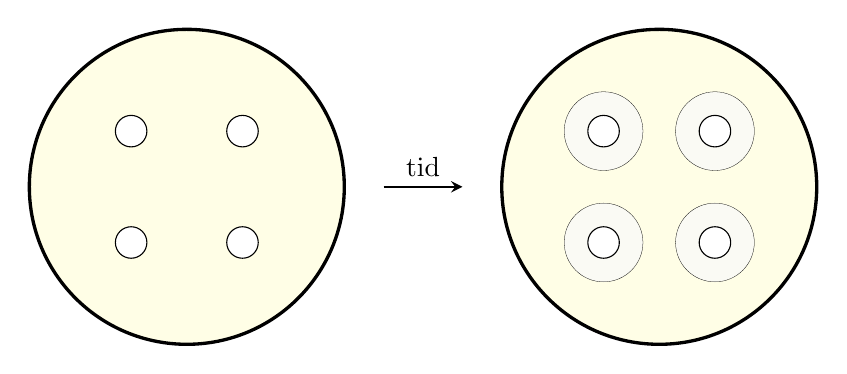
\begin{tikzpicture}
            \filldraw[very thick,fill=yellow!10] (0,0) node(a){} circle (2);
            \filldraw[very thick,fill=yellow!10] (6,0) node(b){} circle (2);

            \draw[-stealth,thick] (2.5,0) -- node[above]{tid} (3.5,0);

            \foreach \x in {45,135,-45,-135}
                \filldraw[fill=gray!5, fill opacity=.75,ultra thin] (b)+(\x:1) circle (0.5);

            \foreach \x in {a,b}
                \foreach \y in {45,135,-45,-135}
                \filldraw[fill=white] (\x)+(\y:1) circle (0.2);
        \end{tikzpicture}
        \caption{Diffusion af stof indeholdt i papirdiske.}
    \end{figure}
    Den vækstfrie radius vil afhænge af antibiotikaens effektivitet, da koncentrationen vil falde i takt med at stoffet diffunderer når længere og længere ud. Med udgangspunkt heri kan et kvalitativt gæt på den minimum inhibitoriske koncentration opstilles.
    \begin{figure}[H]\centering
        \begin{tikzpicture}
            \filldraw[very thick,fill=yellow!10] (0,0) node(a){} circle (2);


            \draw[-stealth,thick] (2.5,0) -- node[above]{vækst} (3.5,0);

            \filldraw[very thick,fill=yellow!10] (6,0) node(b){} circle (2);

            \filldraw[pattern={Lines[angle=45,distance=1.5mm]},pattern color=black] (6,0) circle (1.99);

            \filldraw[fill=yellow!10,very thin] (b)+(45:1) circle (0.3);
            \filldraw[fill=yellow!10,very thin] (b)+(135:1) circle (0.75);
            \filldraw[fill=yellow!10,very thin] (b)+(-135:1) circle (0);
            \filldraw[fill=yellow!10,very thin] (b)+(-45:1) circle (0.5);

            \foreach \x in {a,b}
                \foreach \y in {45,135,-45,-135}
                \filldraw[fill=white] (\x)+(\y:1) circle (0.2);

            \node[font=\footnotesize] at (.71,.71) {$c$};
            \node[font=\footnotesize] at (.71,-.71) {$d$};
            \node[font=\footnotesize] at (-.71,.71) {$a$};
            \node[font=\footnotesize] at (-.71,-.71) {$b$};

            \node[font=\footnotesize] at (6.71,.71) {$c$};
            \node[font=\footnotesize] at (6.71,-.71) {$d$};
            \node[font=\footnotesize] at (5.29,.71) {$a$};
            \node[font=\footnotesize] at (5.29,-.71) {$b$};

        \end{tikzpicture}
        \caption{Illustration af hæmningsradius. MIC: $b>c>d>a$.}
    \end{figure}
    Det samme princip benyttes her med parabenerne. En relativt koncentreret parabenopløsning bestående af ethanol og paraben fremstilles hvorefter de sterile papirdiske vædes deri, de stilles herefter til tørring for at minimere ethanolens egen bakteriehæmmende virkning. Papirdiskene placeres på en poddet Hueller--Minton--agarplade, hvorefter de let præsses ned på agarpladen med en flamme--steriliseret pincet for at sikre overfladekontakt. Pladerne stilles herefter til inkubering natten over, hvorefter radius af de hæmmende zoner måles.

    \subsubsection{Fortyndingsrække}
    Modsat agar--diffusion benyttes fortyndingsrækker til at bestemme definitive værdier for den minimale inhibitoriske koncentration for forskellige antibakterielle midler (antibiotika, konserveringsmidler, osv.). 

    Dette gøres ved at opstille en fortyndingsrække i et bakteriefyldt medie med det antibaktierelle stof man ønsker at undersøge. Ved at have forskellige koncentrationer af stoffet, og herefter følge udviklingen i OD600 over tid, kan man undersøge hvordan de forskellige koncentrationer påvirker bakterievæksten.
    \begin{figure}[H]\centering
        \begin{tikzpicture}
            \fill[blue!99.9] (-3,.5) rectangle ++(1,-.5) (-3,0) to[bend right=90,looseness=1.25] (-2,0) (-2.5,.5) ellipse (.5 and .2);
            \fill[blue!88.8] (0,0) rectangle ++(0.4,0.5) (0,0) to[bend right=90, looseness=1.75] ++(0.4,0);
            \fill[blue!77.7] (1.25,0) rectangle ++(0.4,0.5) (1.25,0) to[bend right=90, looseness=1.75] ++(0.4,0);
            \fill[blue!66.6] (2.5,0) rectangle ++(0.4,0.5) (2.5,0) to[bend right=90, looseness=1.75] ++(0.4,0);
            \fill[blue!55.5] (3.75,0) rectangle ++(0.4,0.5) (3.75,0) to[bend right=90, looseness=1.75] ++(0.4,0);
            \fill[blue!44.4] (5,0) rectangle ++(0.4,0.5) (5,0) to[bend right=90, looseness=1.75] ++(0.4,0);
            \fill[blue!33.3] (6.25,0) rectangle ++(0.4,0.5) (6.25,0) to[bend right=90, looseness=1.75] ++(0.4,0);
            \fill[blue!22.2] (7.5,0) rectangle ++(0.4,0.5) (7.5,0) to[bend right=90, looseness=1.75] ++(0.4,0);
            \fill[blue!11.1] (8.75,0) rectangle ++(0.4,0.5) (8.75,0) to[bend right=90, looseness=1.75] ++(0.4,0);
            
            \draw[-,thick] (-3,1.5) -- (-3,0) (-2,0) -- (-2,1.5) (-3,0) to[bend right=90,looseness=1.25] node[below]{Parabenopløsning} (-2,0) (-3,0) to[bend left=90,looseness=1.25,opacity=.5] (-2,0);
            \draw[thick] (-2.5,1.5) ellipse (0.5 and 0.25) node(a)[above];
            \draw[thick,opacity=.4] (-2.5,.5) ellipse (.5 and .2);
            \draw[-stealth,thick] (a) to[bend left=75,looseness=1.25] node[above,font=\footnotesize]{$100\si{\mu L}$} (0,2.25)

            \draw[-,densely dotted,thick] (-.5,.5) node[left,font=\footnotesize]{$100\si{\mu L}$} --  (9.65,.5);
            
            \foreach \x in {0,1.25,...,8.75}{
                \draw[thick] (\x,0) --  ++(0,2);
                \draw[thick] ($(\x+0.4,0)$) -- ++(0,2);
                \draw[-,thick] (\x,0) to[bend right=90,looseness=1.75] ++(0.4,0);
                \draw[thick] ($(\x+0.2,2)$) ellipse (.2 and .1);
            }

            \foreach \x in {0.4,1.65,...,8.25}
            \draw[-stealth,thick] (\x,2.25) to[bend left=90,looseness=1.25] node[above,font=\footnotesize]{$100\si{\mu L}$} ++(.85,0);
            }
        \end{tikzpicture}
        \caption{Fortynding ved gentagen overførsel fra brønd til brønd.}
    \end{figure}

    Dette medfører en halvering af koncentrationen fra brønd til brønd beskrevet ved rekursionsligningen:
    \[
        c_n=c_{\text{opløsning}}\cdot 0.5^n, n \in \left\{1,2,3,...,n\right\}
    \]
    Vi opstiller nu en fortyndingsrække hvor den 6.\ brønd svarer til MIC
    \[
        1.25\si{mg\per mL}=c_{\text{opløsning}}\cdot 0.5^6 \Leftrightarrow c_{\text{opløsning}}=\frac{1.25\si{mg\per mL}}{0.5^6}=80\si{mg\per mL}
    \]
    Da det er nødvendigt at vente på at ethanolen fordamper, ønsker vi at nå den nødvendige koncentration med så lille en mængde ethanol som muligt. En mættet opløsning af ethylparaben i ethanol indeholder $550\si{mg\per mL}$, dvs.\ at det må være nødvendigt at overføre:
    \[
        160\si{mg}=550\si{mg\per mL} \cdot V_{\text{ethanol}} \Leftrightarrow V_{\text{ethanol}}=\frac{160\si{mg}}{550\si{mg\per mL}}=290\si{\mu L}
    \]
    Da vi arbejder med en brøndvolumen på $100\si{\mu L}$ benytter vi en 10.\ del af dette. En fortyndingsrække opstiles derfor ved at fylde brøndene med $29\si{\mu L}$ ren ethanol, hvorefter det fortyndes med den mættede opløsning.

    De samme beregninger udføres for propylparaben hvorved vi har at:
    \[
        160\si{mg}=746\si{mg\per mL} \cdot V_{\text{ethanol}} \Leftrightarrow V_{\text{ethanol}}=\frac{160\si{mg}}{746\si{mg\per mL}}=210\si{\mu L}
    \]
    Altså benyttes $21\si{\mu L}$ under opstillingen af propylfortyndingsrækken.

    Efter ethanolen i brøndene er fordampet er vi efterladt med de korresponderende mængder af paraben. Måling af MIC ved svært opløselige produkter kan være svært, da det i praksis medfører at vi vil have et lag uopløst paraben liggende i bunden af brønden, selv ved MIC i teorien da den befinder sig over begge parabeners opløselighed i vand. 

    Dog er der nogle faktorere der medfører at opløseligheden ``stiger'' i praksis. Bl.a. parabenernes evne til at reagere med de lipide bakteriecellemembraner, hvilket medfører en større opløselighed i mediet, samt at OD600--målingerne foregår ved højere temperatur (inkubationstemperatur, $37\si{\degree C}$) end stuetemperatur.
